\documentclass{article}
\usepackage[polish]{babel}
\usepackage[T1]{fontenc}
\usepackage[utf8]{inputenc}
\usepackage{graphicx}
\usepackage{float}
\usepackage[bottom=1.5cm, right=2.5cm, left=2.5cm, top=1.5cm]{geometry}
\graphicspath{{../pliki}}



\title{%
  Cyberbezpieczeństwo - laboratoria 7 \\
  \large Zastosowania kryptografii}
\author{Patryk Łuszczek 272707}
\date{\today}
\begin{document}
\maketitle
\newpage

\section*{1.1 Generowanie kluczy}

\begin{figure}[H]
    \centering
    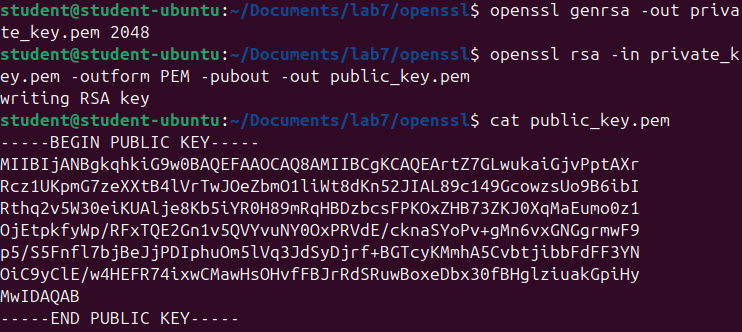
\includegraphics[width=0.5\textwidth]{openssl_pub_key.png}
    \caption{klucze OpenSSL}
\end{figure}

\begin{figure}[H]
    \centering
    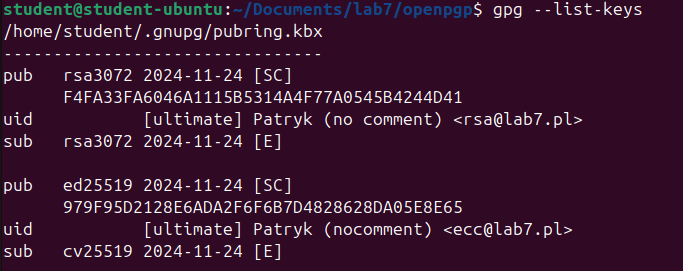
\includegraphics[width=0.5\textwidth]{openpgp_list_keys.png}
    \caption{klucze OpenPGP}
\end{figure}

\section*{1.2 Eskport klucza publicznego}
Wszystkie klucze zostały wyeksportowane pomyślnie.
\section*{1.3 Przeniesienie kluczy publicznych}
Klucze publiczne zostały przeniesione na maszynę wirtalną Kali.
\section*{1.4 Importowanie kluczy}
Wszystkie klucze zostały zaimportowane pomyślnie, przy imporcie kluczy OpenPGP należy je podpisać własnym kluczem lokalnym.

\begin{figure}[H]
    \centering
    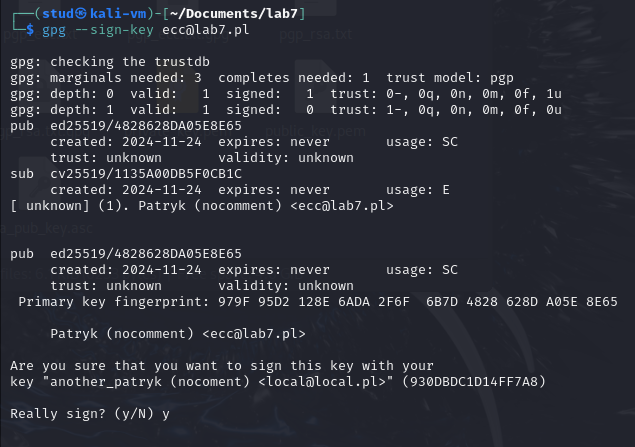
\includegraphics[width=0.5\textwidth]{sign_imported_key.png}
    \caption{Podpisanie klucza OpenPGP}
\end{figure}

\textbf{Fingerprints}
\begin{figure}[H]
    \centering
    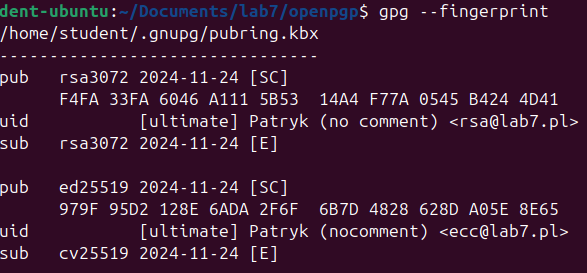
\includegraphics[width=0.5\textwidth]{ubuntu_fingerprint.png}
    \caption{Odcisk palca kluczy na koncie "nadawcy"}
\end{figure}

\begin{figure}[H]
    \centering
    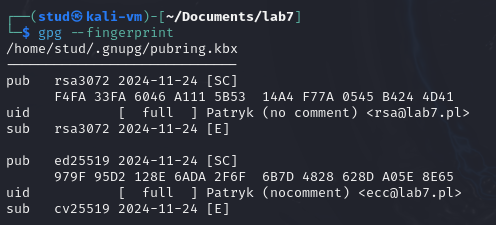
\includegraphics[width=0.5\textwidth]{fingerprint_kali.png}
    \caption{Odcisk palca kluczy na koncie "odbiorcy"}
\end{figure}




\section*{1.5 Podpisanie pliku tekstowego}

\begin{figure}[H]
    \centering
    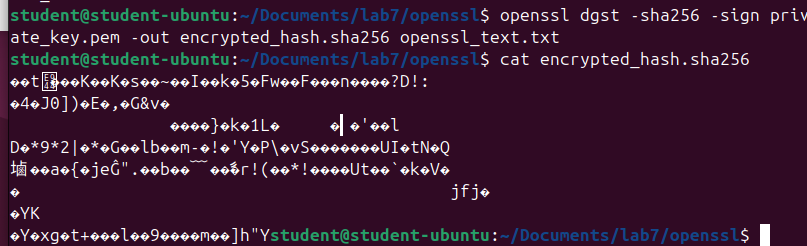
\includegraphics[width=0.5\textwidth]{openssl_signed.png}
    \caption{Plik podpisany za pomocą OpenSSL}
\end{figure}


\begin{figure}[H]
    \centering
    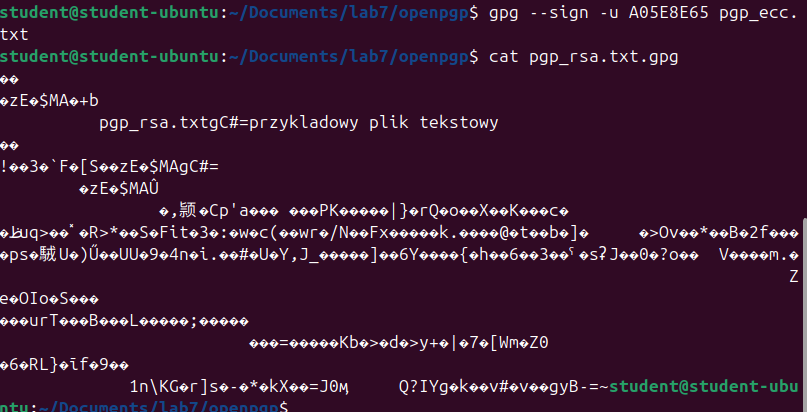
\includegraphics[width=0.5\textwidth]{openpgp_signed_ecc.png}
    \caption{Plik podpisany za pomocą OpenPGP RSA}
\end{figure}

\begin{figure}[H]
    \centering
    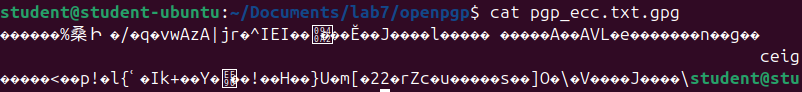
\includegraphics[width=0.5\textwidth]{signed_ecc.png}
    \caption{Plik podpisany za pomocą OpenPGP ECC}
\end{figure}


\section*{1.6 - 1.7 Weryfikacja podpisów oraz zmiana zawartości}
Każdy podpis został pierw zweryfikowany. Po pomyślnej weryfikacji została zmieniona zawartość oryginalnego pliku tekstowego (w przypadku OpenSSL), oraz pliku podpisanego za pomocą OpenPGP.
Weryfikacja podpisów po zmianie zawartości pliku tekstowego zakończyła się zwróceniem błędu.

\begin{figure}[H]
    \centering
    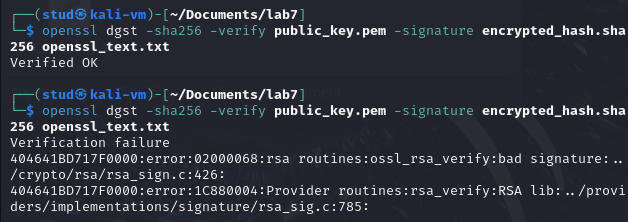
\includegraphics[width=0.5\textwidth]{openns_verify.png}
    \caption{Weryfikacja OpenSSL}
\end{figure}


\begin{figure}[H]
    \centering
    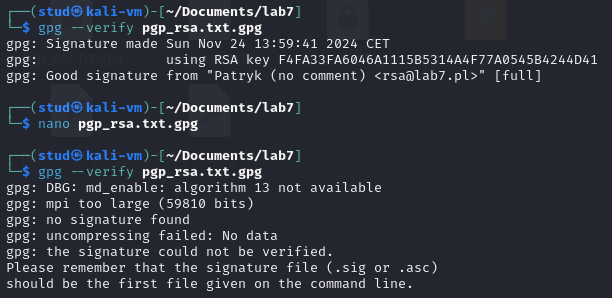
\includegraphics[width=0.5\textwidth]{gpg_verify_rsa.png}
    \caption{Weryfikacja OpenPGP RSA}
\end{figure}

\begin{figure}[H]
    \centering
    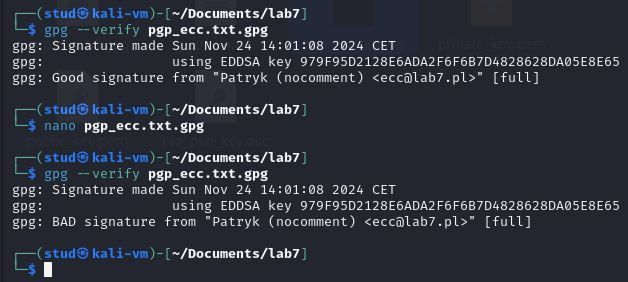
\includegraphics[width=0.5\textwidth]{gpg_verify_ecc.png}
    \caption{Weryfikacja OpenPGP ECC}
\end{figure}

\section*{1.8 Szyfrowanie OpenPGP}

W celu szyfrowania zostały wykorzystane dwa pliki o jednakowej zawartości "przykładowy plik tekstowy".
Następnie pliki zostały odszyfrowane. Można zauważyć, że zawartość po odszyfrowaniu jest taka sama jak przed szyfrowaniem.
Następnym krokiem była próba zmieniania zawartości zaszyfrowanego pliku oraz jego odszyfrowanie.
Operacja zakończyła się niepowodzeniem dla obu zaszyfrowanych plików ze zmienioną zawarością.

\begin{figure}[H]
    \centering
    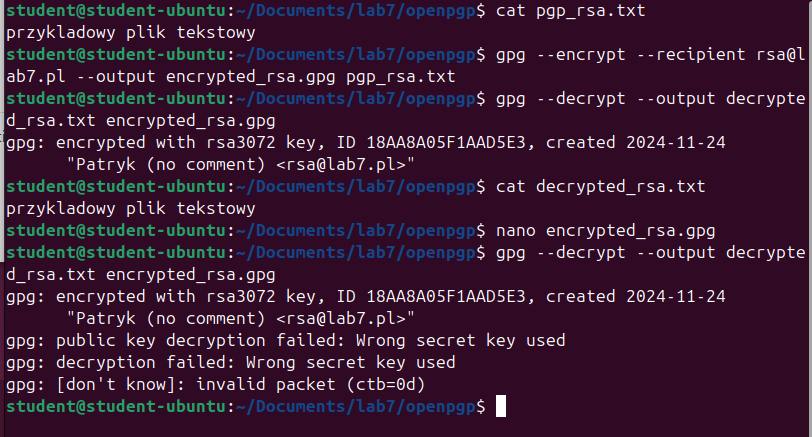
\includegraphics[width=0.5\textwidth]{decrypt_rsa.png}
    \caption{Szyfrowanie i deszyfrowanie OpenPGP RSA}
\end{figure}



\begin{figure}[H]
    \centering
    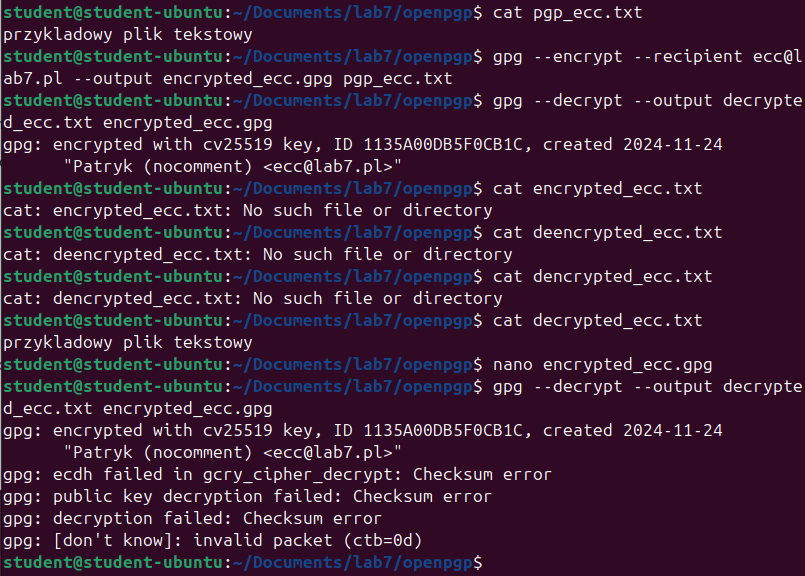
\includegraphics[width=0.5\textwidth]{decrypt_ecc.png}
    \caption{Szyfrowanie i deszyfrowanie OpenPGP ECC}
\end{figure}



\section*{1.9 Czy można wygenerować tylko jeden z pary kluczy dla algorytmów
  asymetrycznych (np. klucz prywatny)? Czy to miałoby sens?}

Generowanie jedynie jednego z kluczy nie jest możliwe, ponieważ są one ze sobą ściśle powiązane. Dodatkowo generowanie tylko jednego z nich nie miałoby sensu,
ponieważ uniemożliwiałoby to wykorzystanie własności kryptografii asymetrycznej, która wymaga użycia dwóch różnych kluczy.
Tak więc, każdy z nich ma swoje zastosowanie. Dla przykładu klucz prywatny jest wykorzystywany do odszyfrowywania wiadomości oraz podpisywania ich, natomiast klucz publiczny służy do szyfrowania i weryfikacji plików.

\section*{1.10 Jaką formę ma klucz GPG? Czym różni się klucz PEM od klucza OpenPGP?}

Główną różnicą między kluczem GPG a kluczem PEM jest zawartość metadanych w kluczu GPG.
Przechowuje on informacje o właścicielu klucza oraz date ważności.


\section*{1.11 Czy wymiana kluczy prywatnych jest uzasadniona?}

Klucz prywatny, jak sama nazwa wskazuje, powinien pozostać sekretnym kluczem jego twórcy. Wymiana kluczy prywatnych jest nieuzasadniona i może prowadzić do
niepożądanych konsekwencji. Każdy kto przechwyci nasz klucz prywatny będzie mógł się pod nas "podszyć" np. podpisując wiadomości w naszym imieniu.

\section*{1.12 Jaki rezultat został osiągniety w zadanie 1.7 i dlaczego ?}

Po zmodyfikowaniu treści dokumentu podpis nie mógł zostać zweryfikowany pomyślnie.
Przyczyną porażki weryfikacji jest fakt, że podczas modyfikacji pliku, zmienia się wartość hashu, który przestaje być zgodny z z podpisem.

\section*{1.13 Co to jest odcisk palca?}

Odcisk palca jest "skrótem" klucza publicznego. Używany jest w celach łatwej identyfikacji klucza, dzięki bardziej "przyjaznej" dla użytkownika postaci.

\section*{1.14 Czy udało ci się zmienić jeden znak w zaszyfrowanym pliku i odszyfrować zaszyfrowany
  tekst? Odpowiedź uzasadnij.}

Zmiana zawartości pliku zaszyfrowanego skutkuje utratą możliwości do jego ponownego odszyfrowania.
Dzieje się tak dlatego, że została naruszona struktura i integralność danych. Te "blędy" w pliku są wykrywane przez różne mechanizmy
kontroli integralności pliku (np. checksum), które odrzucają plik.

\section*{1.15 Jaka jest różnica w sygnaturze (OpenPGP) dla algorytmu ECC i RSA?}

Różnica między tymi dwoma sygnaturami leży przede wszystikm w sposobie ich generowania oraz rozmiarze zapewniającym dostateczne bezpieczeństwo.
Dla domyślnych wartości proponowanych przez OpenPGP zostały wygenerowe sygnatury dla ECC oraz RSA. Można zauważyć, że sygnatura ECC jest znacznie mniejsza i bardzie "kompaktowa" niż RSA.
Dodatkowo generowanie kluczy ECC jest szybsze niż generowanie ich dla RSA. Generowanie sygnatur za pomocą ECC odbywa się za pomocą krzywych eliptycznych, które pozwalają na osiągniecie takiego samego poziomu bezpieczeństwa
jak RSA przy znacznie mniejszych rozmiarach. W przypadku RSA, sygnatury są generowany na podstawie dużych liczb pierwych, a rozmiar rośnie wykładniczo wraz ze wzrostem wymaganego poziomu bezpieczeństwa.

\section*{1.16 Czy wiadomość może być podpisana kluczem publicznym? Jeśli tak, jakie mogą
  być konsekwencje}

Domyślnie szyfrowanie odbywa się z wykorzystaniem klucza prywatnego. Gwarantuje to, że tylko osoba posiadająca klucz prywatny będzie w stanie podpisać plik, czy zaszyfrować wiadomość "w swoim imieniu".
Jeśli natomiast wykorzystamy klucz publiczny do szyfrowania, każdy posiadający ten klucz publiczny będzie mógł podpisać wiadomość w naszym imieniu, więc tak naprawde nie będzie możliwa autoryzacja
nadawcy wiadomości.
\end{document}